\chapter{Implementierung}

Die Implementierung ist in drei Teile gegliedert. Zu Beginn wird gezeigt wie mit Python und der \textit{opencv}-Biblitohek Gradienten von Bildern erzeugt wurden. Diese stellen die Basis für den zweiten Schritt, der Komprimierung durch einen Autoencoder dar. Die Verarbeitung kann an dieser Stelle ohne technischen Bruch fortfahren, da der Autoencoder in TensorFlow und somit ebenfalls in Python umgesetzt wurde. Die so erzeugten komprimierten Features werden zunächst zwischengespeichert, da sie nicht direkt weiterverarbeitet werden können: Der Bag of Visual Words wurde direkt in CUDA C umgesetzt und muss daher die Features wieder einlesen. Ursprünglich war die Implementierung des gesamten Projektes in CUDA geplant. Der Aufwand für die Implementierung des gesamten Modells, insbesondere den Autoencoder, bzw. neuronale Netze im Allgemeinen, geht leider über den Rahmen dieser Arbeit hinaus. 

\section{Extraktion der Features}

Zu Ermittlung der \textit{keypoints} durch den SIFT-Detektor wird auf die \textit{opencv}\footnote{https://github.com/opencv/opencv} Implementierung von SIFT zurückgegriffen. Zur Verwendung des SIFT Algorithmus ist es erforderlich das \textit{opencv} Projekt zusammen mit dem \textit{opencv-contrib}\footnote{https://github.com/opencv/opencv-contrib} Projekt selbst zu kompilieren. Bei SIFT handelt es sich um einen patentierten Algorithmus, daher ist er seit Version 3.0 nicht mehr standardmäßig im \textit{opencv} Projekt enthalten.

Da der Autoencoder in Python geschrieben ist, erfolgt die Gewinnung der Patches in der gleichen Sprache, um so eine einfache weitere Verarbeitung zu ermöglichen. Der Prozess lässt sich in drei Schritte untergliedern. Um alle Features eines Bildes zu erhalten, wird die Funktion \textit{extractFeatures} mit dem Pfad zu einer Bilddatei ausgerufen. Es wird das Bild eingelesen, konvertiert und durch den \textit{opencv} SIFT-Detektor die \textit{keypoints} ermittelt. Die Berechnung der Gradienten der Nachbarschaften um diese \textit{keypoints} erfolgt dann durch die Funktion \textit{computeDescriptors}:

\lstset{language=Python}
\begin{lstlisting}
def computeDescriptors(image, keypoints):
  descriptors = []
  
  for keypoint in keypoints:
  	patch = getPatch(image, keypoint)
  	gradients = computeGradients(patch)
  	descriptors.append(gradients)
  return descriptors
  
def getPatch (image, keypoint):
  x, y = keypoint.pt[0], keypoint.pt[1]
  return image[y-20:y+21, x-20:x+21]
\end{lstlisting}

Für jeden \textit{keypoint} werden nun wiederum \textit{Patches} berechnet: Hierbei handelt es sich um die Nachbarschaften der Größe $41 \times 41$. Die Gradienten in vertikale und horizontale Richtung eines solchen \textit{Patches} werden durch \textit{computeGradients} bestimmt. In Zeile 2 und 3 in Abbildung \ref{lst:compGrad} findet die Konvolution des Patches mit einem Sobel-Operator statt, den \textit{opencv} anbietet.

\lstset{language=Python,label={lst:compGrad}}
\begin{lstlisting}
def computeGradients(image):
  grad_x = cv2.Sobel(image, cv2.CV16S, 1, 0)
  grad_y = cv2.Sobel(image, cv2.CV16S, 0, 1)
  return [grad_x, grad_y]
\end{lstlisting}

In Abbildung \ref{img:gradients} sind auf der rechten Seite sind, in zwei Reihen, einige der gefundenen Gradienten des Bildes auf der linken Seite dargestellt. Dadurch, dass das Bild des Stop-Schildes viele deutliche Kanten aufweist, sind die Gradienten leicht zuzuordnen.

\begin{figure}
	\centering
	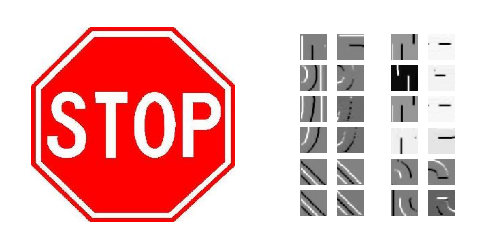
\includegraphics[scale=0.65]{images/gradients_patch.png}
	\caption{Stop-Schild und Gradienten um einige der gefundenen \textit{keypoints}.}
	\label{img:gradients}
\end{figure}

Sollte im späteren eine Umsetzung des Autoencoders in CUDA C erfolgen, so lässt sich die Gewinnung der Patches leicht portieren. Die Verwendung von SIFT erfolgt in C analog (in entsprechender Syntax).

\section{Autoencoder}

In diesem Abschnitt wird behandelt wie der Autoencoder in Python und TensorFlow umgesetzt wurde. Hierfür wird zunächst eine Übersicht über die Projektstruktur gegeben und anschließend wird an Programmcode demonstriert, wie der vov Zhao entworfene Autoencoder abgebildet werden kann.

\subsection{Projektstruktur} Das Python-Projekt für des Autoencoders besteht aus fünf Dateien. In autoencoder.py ist eine gleichnamige Klasse zur objektorientierten Verwendung enthalten. Die Funktionen zur Feature-Extraktion sind in der Datei feature\textunderscore extractor.py und werden im folgenden Abschnitt näher behandelt. Die Datei util.py stellt eine Sammlung allgemein verwendeter Funktionen bereit, z.B. zur Messung von Zeit oder Konvertierung von Datenstrukturen. Wie beim Bag of Visual Words liegt hier eine main-Datei bei, welche die Benutzung des Autoencoders durch die Kommandozeile erlaubt.

\dirtree{%src
.1 src.
.2 autoencoder.py.
.2 feature\textunderscore extractor.py.
.2 main.py.
.2 test.cpp.
.2 util.py.
}

\subsection{Modell in TensorFlow}

Zur Implementierung des Autoencoders wurde TensorFlow verwendet. TensorFlow ist ein DeepLearning Framework und bietet Schnittstellen in diversen Sprachen an. Neben OpenCL wird auch NVIDIAs CUDA unterstützt, sodass TensorFlow Programme automatisch von Grafikkarten profitieren können, ohne das der Entwickler diese explizit berücksichtigen muss. Für diese Umsetzung eines Autoencoders wurde Python und das Projekt \textit{libsdae-autoencoder-tensorflow}\footnote{https://github.com/rajarsheem/libsdae-autoencoder-tensorflow} von Rajarshee Mitra genutzt. Unter Berücksichtigung der bekannten Parameter aus dem Konzept, ergibt sich die folgende Definition eines Modells.

\lstset{language=Python}
\begin{lstlisting}
from deepautoencoder import StackedAutoEncoder
import cv2
import numpy

model = StackedAutoEncoder(
  dims=[3042, 1024, 512, 128, 36],
  activations=['relu', 'relu', 'relu', 'relu', 'relu'], 
  epoch=[1000, 1000, 700, 700, 500], 
  loss='rmse', 
  lr=0.02, 
  batch_size=100
)

def train(features):
  model.fit(features)

def encode(features):
  model.transform(data=features, mode='encode')
  
def decode(features):
  model.transform(data=features, mode='decode')
\end{lstlisting}


In den Zeilen 5 bis 12 findet die Definition des Autoencoders statt. Der \textit{StackedAutoEncoder} entstammt hierbei dem Eingangs erwähnten Projekt von Rajarshee Mitra. In \textit{dims} wird die Menge der Schichten des Encoder-Teils durch eine Liste von Ganzzahlen dargestellt: Eine Zahl steht für die Anzahl der Neuronen pro Schicht. Hier wird davon ausgegangen, dass benachbarte Schichten voll verbunden sind. Der Decoder-Teil ist umgekehrt aufgebaut, daher leitet sich dieser aus der Encoder-Definition ab und muss nicht notiert werden. Folglich werden in \textit{activations} die Aktivierungsfunktion auch nur einmal notiert. 
Die Abkürzung \textit{relu} steht hier für \textit{Rectified Linear Unit (ReLU)}. Die Schichten können über verschiedene Aktivierungsfunktionen miteinander verbunden sein, hier wird aber für alle die \textit{ReLU} benutzt.
Die Liste \textit{epoch} enthält die Anzahl der Trainingsiteration für die Autoencoder, die aus den benachbarten Schichten konstruiert und einzelnen trainiert werden. In Zeile 9 wird unter \textit{loss} die die Metrik definiert, mit welcher der Fehler der Rekonstruktion gemessen wird. \textit{rmse} steht für \textit{root-mean-square error} und ist somit der gemittelte quadratische Fehler. 
Die Lernrate wird hier mit \textit{lr} bezeichnet und wurde entsprechend des konzipierten Autoencoders auf 2\% gesetzt.\newline
In Zeile 14, 17 und 20 werden die Methoden \textit{train}, \textit{encode} und \textit{decode} definiert. Diese stellen die im Entwurf vorgestellten Methoden vor und ermöglichen eine Verwendung des konkreten Autoencoders. Der Parameter \textit{features} muss bei \textit{train} und \textit{encode} eine Liste sein, die als Elemente Listen mit 3042 Komponenten enthält. Konkret werden hier \textit{numpy} Arrays verwendet, sodass sich die Form \textit{shape(n, 3042)} bei $n$ Features ergibt. Dementsprechend erwartet \textit{decode} ein Array der Form \textit{shape(n, 36)}.\newline

Die Datei \textit{main.py} importiert dann den Feature-Extraktor sowie den parametrierten Autoencoder. In Zeile 6 und 7 werden durch die \textit{readImages} Methode die Bilddaten eingelesen. Hierfür müssen die Pfade zu den Trainigs- bzw. Test-Dateien auf der Kommandozeile angegeben werden: \textit{python3 main.py /train/path test/path}. In Zeile 9 wird dann die \textit{train}-Methode des Autoencoders genutzt, um die Gewichte anhand der Trainingsdaten zu initialisieren. In Zeile 10 erfolgt die Komprimierung der Testdaten und abschließend in der nächsten Zeile die Speicherung.

\lstset{language=Python}
\begin{lstlisting}
import sys
import util
import featureExtractor
import autoencoder

train = util.readImages(sys.argv[1])
test = util.readImages(sys.argv[2])

autoencoder.train(featureExtractor.extractAll(train))
result = autoencoder.encode(featureExtractor.extractAll(test))
util.writeFeatures(result)
\end{lstlisting}

\section{Bag of Visual Words}

Zunächst wird eine Übersicht über die Projektstruktur der Bag of Visual Words Implementierung gegeben. Neben der konkreten Klassenstruktur wird auf Abweichungen zum Konzept eingegangen. Dem schließt die Betrachtung des k-means Clustering der Features an, sowie Unterschiede und Limitierungen der \textit{global} bzw. \textit{shared memory} Varianten.

\subsection{Projektstruktur}

Der Bag of Visual Words ist als Klasse in C++ umgesetzt worden und ist auch die öffentliche API des Programms. Der k-means und Histogramm Algorithmus sind CUDA C Programme und tragen somit die Endung .cu. Neben den CUDA Programmen sind hier aber auch Varianten in C zur Ausführung auf CPUs enthalten. In der util.cpp Datei sind Funktionen zur Messung von Ausführungszeiten, Lesen / Schreiben von Dateien und und Formatierung von Zeichenketten enthalten. Zur direkten Ausführung im Projekt ist eine main.cpp Datei enthalten. Hier werden Argumente der Kommandozeile geparst, um einen entsprechenden Bag of Visual Words zu generieren bzw. auszuführen. Inklusive header-Dateien ergibt sich somit folgender Aufbau des src-Ordners:
\dirtree{%src
.1 src.
.2 BagOfVisualWords.h.
.2 BagOfVisualWords.cpp.
.2 histogram.h.
.2 histogram.cu.
.2 kmeans.h.
.2 kmeans.cpp.
.2 main.cpp.
.2 shared.h.
.2 shared.cu.
.2 util.cpp.
.1 makefile.
}

\subsection{Abweichungen zum Konzept}

Da CUDA C eine sehr hardwarenahe Sprache ist, obliegt die effiziente Verwendung des Speichers dem Programmierer. Insbesondere auf dem \textit{device} sollte mit dem Speicher genügsam umgegangen werden. Daher weicht die Implementierung von dem vorgestellten Konzept bei den verwendeten Datentypen ab: Statt Objekte für Cluster oder Features zu erzeugen, werden diese Typen einfach als \textit{pointer} von \textit{float}-Werten dargestellt. Dies ist für die Features problemlos möglich, doch die Information über die Mitgliedschaft seiner Features kann nicht länger in einem Cluster enthalten sein. Diese Informationen wird stattdessen global vom BagOfVisualWords in der privaten Variablen \textit{membership} gehalten und als \textit{pointer} zu Integer-Werten dargestellt. Diese Liste enthält für jedes Feature den Index des Clusters, dem es zugeordnet ist. Der Index eines Features an der Stelle \textit{i} in der \textit{features} Liste, ist dann an der Stelle $membership_i$ gespeichert.\newline
Dadurch dass \textit{pointer} verwendet werden, erfordern die meisten Funktionsaufrufe nun zusätzliche Parameter: 

\begin{itemize}
	\item Die Anzahl der Features \textit{count} muss angegeben werden. In C ist es nicht auf einfachem Weg möglich zu bestimmen, auf wie viele Elemente ein \textit{pointer} zeigt.
	\item Die Anzahl an Komponenten \textit{featureSize} in einem Feature bzw. Cluster muss angegeben werden. Auch hier handelt es sich wieder um einen \textit{pointer}, daher ist es nicht möglich, die Anzahl der Elemente zu ermitteln.
\end{itemize}

Um Vergleiche mit sequentiellen Varianten zu ermöglichen, kann durch den Aufruf \textit{setMode(mode: Int)} auf einem BagOfVisualWords-Objekt festgelegt werden, ob die GPU (0) oder CPU (1) verwendet werden soll.

\subsection{Paralleler k-means Algorithmus}

Als Referenzimplementierung für die Umsetzung in CUDA C diente hier das Projekt von Serban Giuroiu \footnote{https://github.com/serban/kmeans}. Der \textit{kernel} wurde adaptiert und leicht verändert, um gemeinsam genutzt Methoden auszulagern. Die Funktion \textit{kmeans} in der Datei kmeans.cuda kann genutzt werden, um Clustering auf der GPU auszuführen. Der Algorithmus erwartet dabei als Parameter:

\begin{itemize}
	\item \textbf{float **features} Eine Liste von Feature-Vektoren, die zu gruppieren sind.	
	\item \textbf{float **clusters} Eine Liste, welche mit den Clustern befüllt wird.
	\item \textbf{int *membership} Diese Liste wird die Cluster-Vektor-Zuordnung enthalten. An der Stelle $membership_i$  wird der Index des Clusters aus \textit{clusters} eingetragen, dem das Feature $features_i$ zugeordnet wird.
	\item \textbf{int featureSize} Die Anzahl der Komponenten in einem Feature-Vektor, also die Anzahl der \textit{float}-Werte.	
	\item \textbf{int count} Die Anzahl der Features.
	\item \textbf{int k} Die Anzahl der zu bildenden Cluster $k$.
	\item \textbf{int iterations} Die maximale Anzahl an Iterationen, die durchlaufen wird, falls bisher keine Konvergenz erreicht wurde.
	\item \textbf{float conv} Ein Schwellwert, der in jeder Iteration mit der relativen Veränderung der Mitgliedschaft verglichen wird. Ist er größer, wird das Clustering beendet.
\end{itemize}

Die Datenstruktur der Features und Cluster ist dabei spaltenorientiert, d.h. das \textit{features} und \textit{clusters} jeweils auf \textit{featureSize} viele Elemente zeigen. Dahinter liegen dann im Fall der Features \textit{count} viele \textit{pointer} zu den eigentlichen Koordinaten, im Fall der Cluster \textit{k} viele. An der Stelle \textit{features[0][0]} befindet sich dann die erste Koordinate des ersten Elements, an der Stelle \textit{features[0][1]} die erste Koordinate des zweiten Elements, etc.\newline
Vor dem Aufruf des \textit{kernels} wird für die Features und Cluster der notwendige Speicher allokiert und die Daten zum \textit{device} kopiert. Die Dimensionen der Features sowie der Cluster werden durch \textit{Float}-Werte dargestellt. Ein SIFT Feature-Vektor belegt so $128 \times 4 = 512$ Byte. Der Deskriptor, der durch den Autoencoder erzeugt wurde, belegt $36 \times 4 = 144$ Byte. Da die Features ursprünglich als zweidimensionales Array vorliegen (\textit{pointer-pointer} zu \textit{float}-Werten), werden diese in ein eindimensionales Arrays konvertiert werden, damit die Daten von \textit{host} zu \textit{device} kopiert werden können.\newline
Der Clustering-Vorgang wird nun in einer Schleife durchgeführt. Dabei werden die in der Konzeption vorgestellten Funktionen \textit{computeEuclideanDistance}, \textit{findNearestCluster} und \textit{computeDelta} innerhalb der Schleife nacheinander aufgerufen. Abweichend zum Konzept, erfordern auch diese Funktionen \textit{count} und \textit{featuresSize} als zusätzliche Parameter, um korrekt über die \textit{pointer} iterieren zu können.
Wenn das Konvergenzkriterium \textit{conv} oder die maximale Anzahl an Iterationen \textit{iterations} erreicht wurde, ist der Vorgang beendet und die das Ergebnis wird vom \textit{device} zum \textit{host} in \textit{clusters} respektive \textit{membership} kopiert.

\subsection{Shared memory}

Zur Beschleunigung der Berechnung bei der Suche des nächsten Clusters zu einem gegebenen Punkt, soll CUDAs \textit{shared memory} genutzt werden. Hierfür werden die Cluster pro Block vom \textit{global} in den \textit{shared memory} kopiert. Daraus ergibt sich eine Anpassung an mehreren Stellen im Programm. Um beide Implementierungen zu unterstützen, fragt eine Direktive für den Präprozessor den Wert der Variable \textit{SHARED\textunderscore MEM} ab. Falls der Wert der Variable \textit{true} ist, wird Code nur für die \textit{shared memory} Implementierung eingebunden, andernfalls für die \textit{global memory} Variante:

\lstset{language=C}
\begin{lstlisting}
#if SHARED_MEM
// shared memory Logik
#else
// global memory Logik
\end{lstlisting}

Die Größe des extra zu allokierenden Speichers pro Block muss in \textit{blockSharedDataSize} berücksichtigt werden und ergibt sich aus der Anzahl der Cluster und der Anzahl der Elemente eines Features:

\lstset{language=C}
\begin{lstlisting}
const unsigned int membershipDataSize = numThreads * sizeof(unsigned char);
const unsigned int clusterDataSize = k * featureSize * sizeof(float);

#if SHARED_MEM
    const unsigned int blockSharedDataSize = membershipDataSize + clusterDataSize;
#else
	const unsigned int blockSharedDataSize = membershipDataSize;
\end{lstlisting}

In der Funktion \textit{findNearestCluster} wird der Parameter \textit{clusters} in \textit{deviceClusters} umbenannt. Wenn die \textit{global memory} Variante genutzt wird, sind diese gleich den Clustern \textit{clusters}. Andernfalls werden die \textit{deviceCluster} in die \textit{clusters} im \textit{shared memory} kopiert.

\lstset{language=C}
\begin{lstlisting}
extern __shared__ char sharedMemory[];
unsigned int *membershipChanged = (unsigned int *)sharedMemory;
    
#if SHARED_MEM
    float *clusters = (float *)(sharedMemory + blockDim.x);
	for (int i = threadIdx.x; i < k; i += blockDim.x) {
  		for (int j = 0; j < size; j++) {
    		clusters[k * j + i] = deviceClusters[k * j + i];
  		}
	}
	__syncthreads();
#else
    float *clusters = deviceClusters;
#endif
\end{lstlisting}

Da die Größe von \textit{clusterDataSize} hier von $k$ und $size$ abhängt, also der Anzahl der Cluster und der Anzahl der Komponenten eines Features, ist diese Implementierung nur einsetzbar, wenn $k$ und $size$ in Hinsicht auf den verfügbaren \textit{shared memory} nicht zu groß gewählt werden. Die Größe von \textit{membershipDataSize} ist nur abhängig von der Anzahl der Threads. Werden beispielsweise 256 Threads pro Block gewählt, benötigt dies konstant, unabhängig von $k$ und $size$, 1024 Byte \textit{shared memory}. Für die hier verwendeten Deskriptoren kann somit eine Obergrenze für $k$ berechnet werden. Gängige Modelle Nvidias CUDA kompatibler Grafikkarten sind mit 16 oder 48 Kilobyte \textit{shared memory} ausgestattet. Von 256 Threads pro Block ausgehend ergibt dies ein maximales $k$ von $(memory - 1024) / 512$. Für SIFT sind dies bei 48 Kilobyte maximal 91, für 16 Kilobyte 29 Cluster. Der von Zhao entworfene Deskriptor ermöglicht bei 48 Kilobyte Speicher 326 Clustern, für 16 Kilobyte bis zu 104. Sind dennoch mehr Cluster notwendig, muss auf die \textit{global memory} Implementierung zurückgegriffen werden. Hier werden, je nach Anzahl der Cluster, erheblich höhere Berechnungszeiten erwartet, jedoch gibt es kein Limit für die Gesamtanzahl an Clustern.